% ------------------------------------------------------------------------
% file `main-bookexercise-4-exercise-body.tex'
%
%     exercise of type `bookexercise' with id `4'
%
% generated by the `exercise' environment of the
%   `xsim' package v0.21 (2022/02/12)
% from source `main' on 2026/10/13 on line 1445
% ------------------------------------------------------------------------
    1. 若某哈夫曼树度为2的节点有7个，能否确定度为0的节点有几个？\\

    2. 若某哈夫曼树度为2的节点有7个，能否确定这棵哈夫曼树共有几个节点？\\

    3. 练习：有5个元素A、B、C、D、E的权值分别为1,2,2,4,5，将这五个元素作为叶节点构造一棵哈夫曼树。\\

    4. 下列完全二叉树中，是最小堆的有\underline{\hspace{1.5cm}}，是最大堆的有\underline{\hspace{1.5cm}}。\\[0.5em]
    \begin{center}
        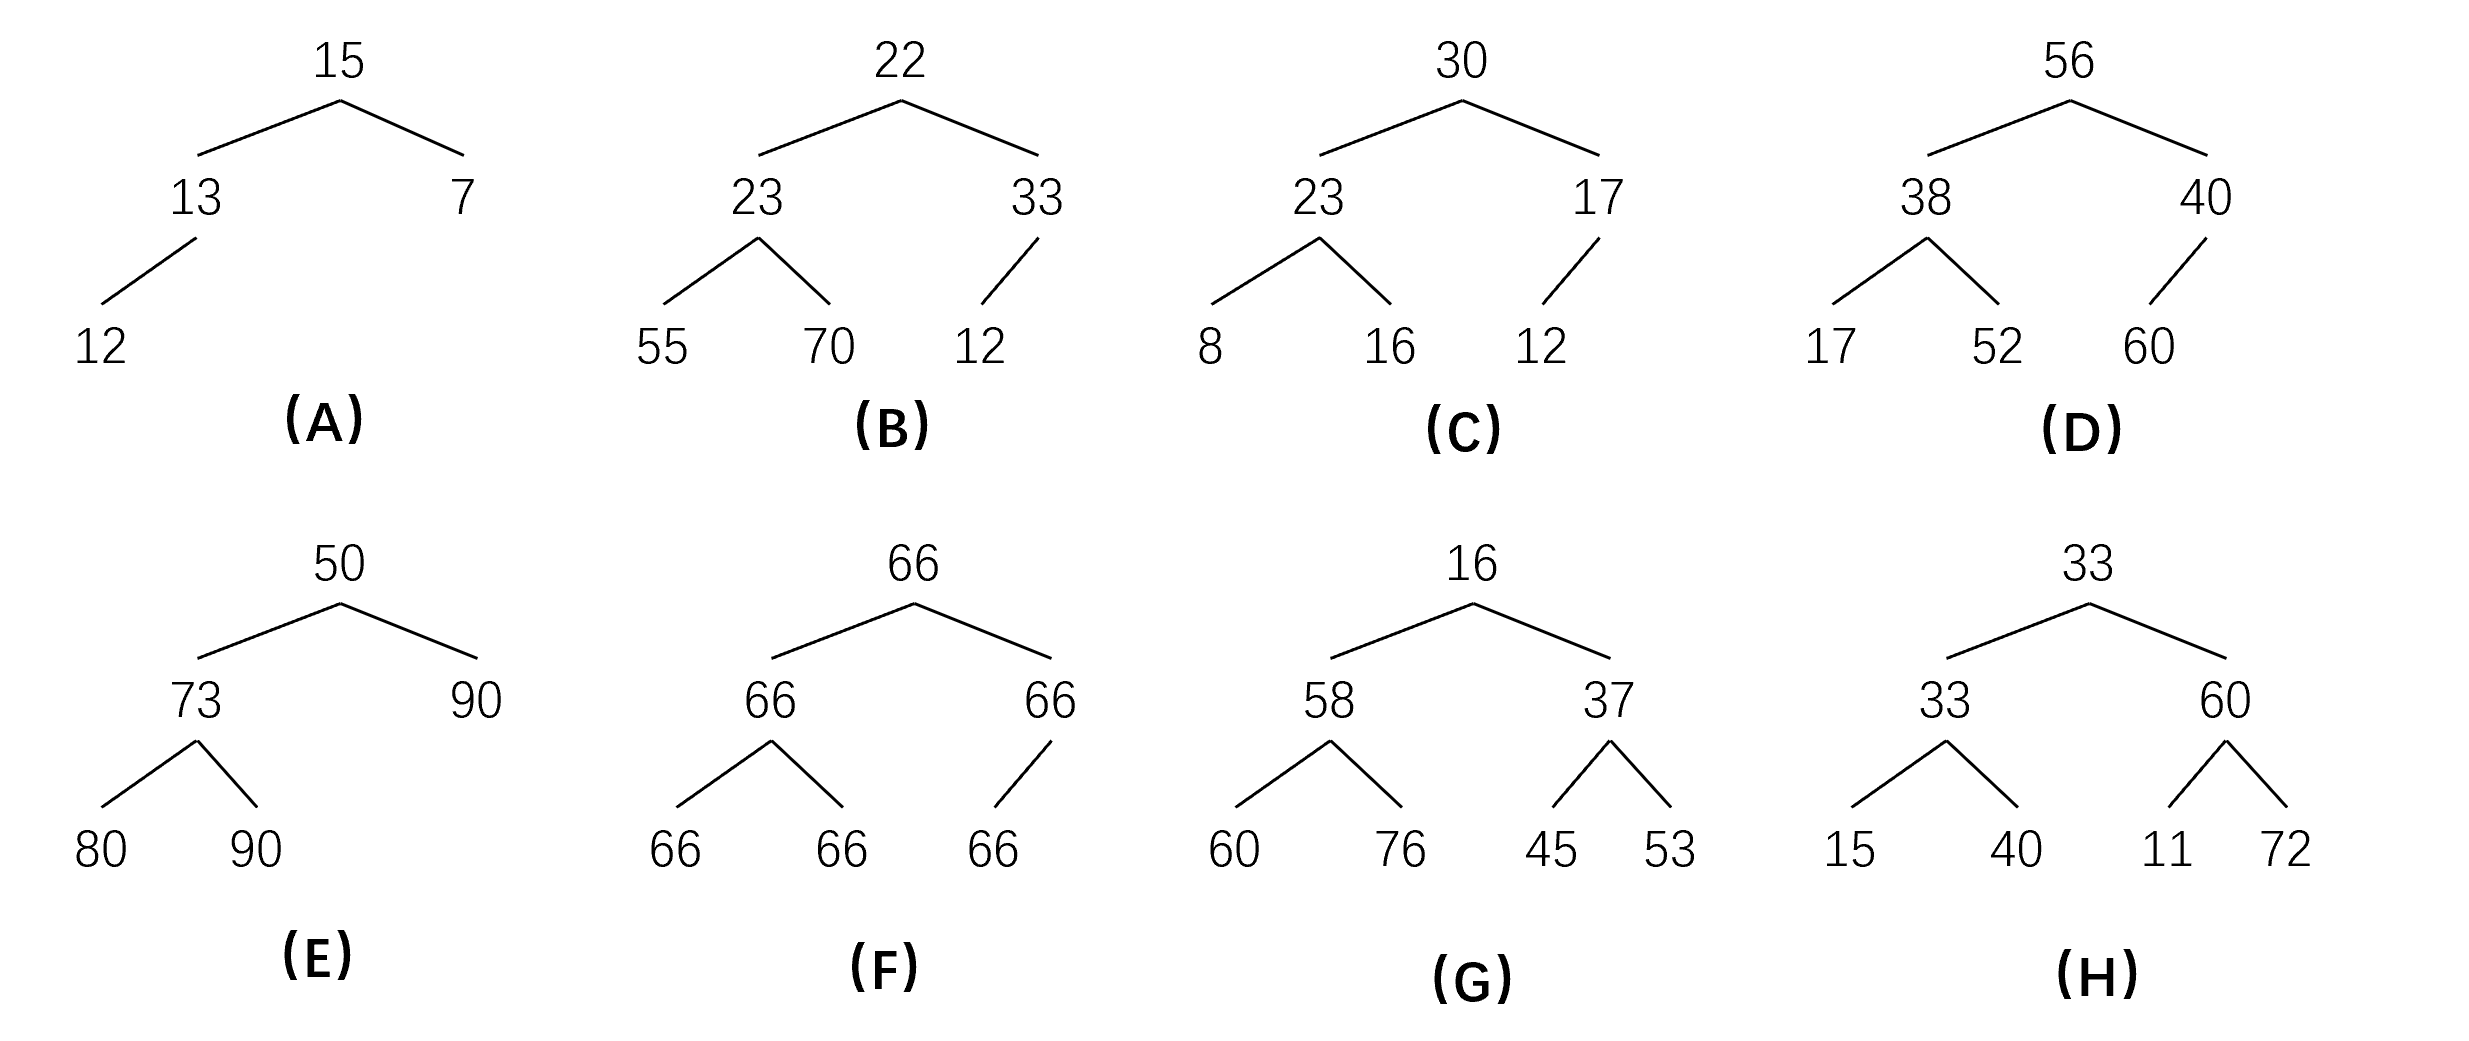
\includegraphics[width=0.88\textwidth]{assets/pics_and_ppts/ch4/习题_判断最大堆和最小堆.png}
    \end{center}

    5. 对于下图所示的二叉树，各节点中的数字表示该节点的权值。下列说法错误的是\underline{\hspace{1cm}}\\[0.5em]
    \begin{center}
        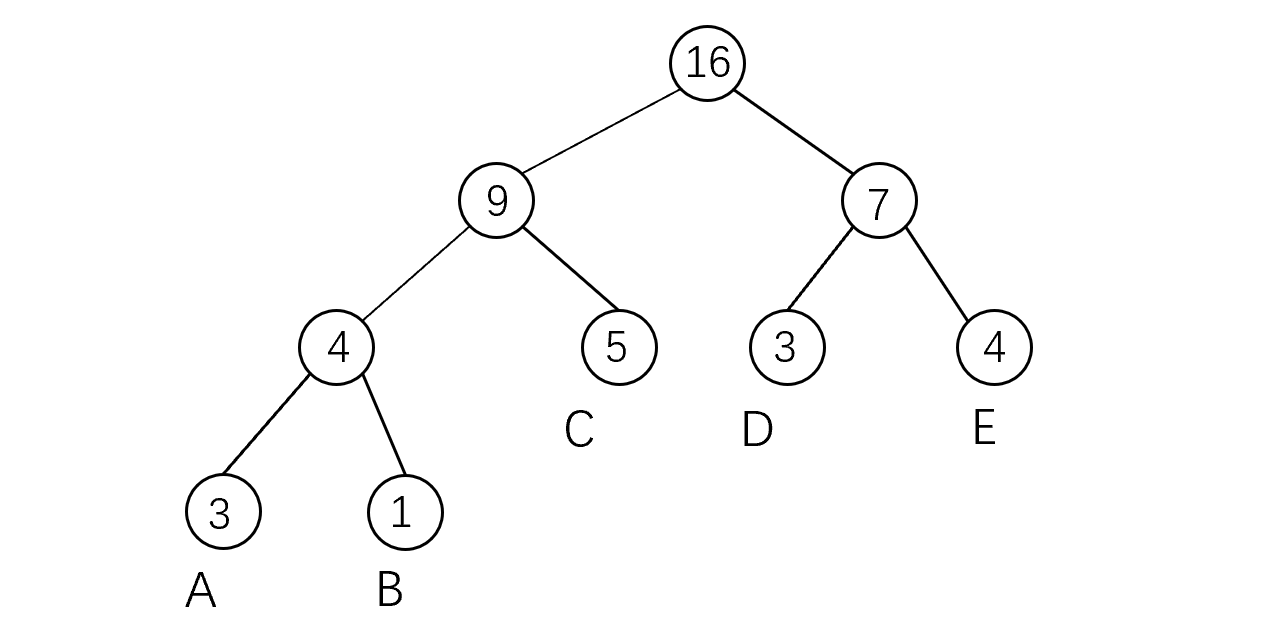
\includegraphics[width=0.57\textwidth]{assets/pics_and_ppts/ch4/习题图_一棵哈夫曼树.png}
    \end{center}

\noindent A. 节点B的带权路径长度为3\\
B. 这棵树的带权路径长度为60\\
C. 以A、B、C、D、E为叶节点构造一棵二叉树，图示的树能使得带权路径长度达到最小\\
D. 以A、B、C、D、E为叶节点构造一棵二叉树，图示的树并不是唯一的带权路径长度最小的树\\

    6. 假设某位同学已经封装好了一个数据结构：priority\_queue，这是一个最小堆，可以通过：
    \begin{bulk}
        priority\_queue<int, vector<int>, greater<int> > min\_heap;
    \end{bulk}
    定义并初始化一个初始为空的，名为min\_heap的最小堆，可容纳int类型元素。其中
    \begin{bulk}
        priority\_queue<int, vector<int>, greater<int> >
    \end{bulk}
    是一种类型，只不过看起来比较长而已。读者大可不必关注其细节，只知道上述代码用该类型定义的min\_heap是一个最小堆，并直接使用相关操作即可。
    min\_heap支持以下操作：
    \begin{enumerate}[label=\arabic*）]
        \item min\_heap.push(value);  // 向堆中插入一个值为value的元素；
        \item int a = min\_heap.top();   // 获取堆顶元素，赋值给a(但不删除堆顶元素)；
        \item min\_heap.pop();       // 删除堆顶元素；
    \end{enumerate}
    对初始为空的minHeap依次执行以下操作，请指出每一次使用min\_heap.top()获取堆顶元素时，获取到的元素值是多少。
    \begin{enumerate}[label=\arabic*）]
        \item min\_heap.push(5);
        \item min\_heap.top();    // 1
        \item min\_heap.push(3);
        \item min\_heap.push(4);
        \item min\_heap.top();    // 2
        \item min\_heap.pop();
        \item min\_heap.top();    // 3
    \end{enumerate}

    \vspace{\baselineskip}

    7. 请你借助{\color{red}\textbf{上题}}给出的priority\_queue及其相关操作来解决“合并柴薪”问题。输入一个长度为n的数组w[]表示各堆柴薪的重量（均为正整数），返回一个正整数，
    表示最优情况下消耗的体力值。
    \begin{cppcode}
        int MinCost(int w[], int n) {
            priority_queue<int, vector<int>, greater<int>> min_heap;
            // 在下方完成你的代码
        }
    \end{cppcode}

    8. （某年408真题）对n个互不相同的符号进行哈夫曼编码，若生成的哈夫曼树共有115个节点，则n的值是\\[0.5em]
    \begin{tabular}{llll}
    A. 56 & B. 57 & C. 58 & D. 60
    \end{tabular}\\

    9. （某年408真题）若某二叉树有5个叶节点，其权值分别为10，12，16，21，30，则其最小的带权路径长度（WPL）是\underline{\hspace{1cm}}\\[0.5em]
    \begin{tabular}{llll}
        A. 89 & B. 200 & C. 208 & D. 289
    \end{tabular}\\



